
\section{Git and Github}
\subsection{Brief description}
\href{https://en.wikipedia.org/wiki/Git_(software)}{Git} is "a version control system that is used for system development". Not only can it keep track of all the changes imparted to code undergoing development by a single user, but its functionalities are extremely handy when several developers interact with the same piece of code concurrently.\\
\href{https://github.com/}{Github} is a website that offers a server architecture that you can synchronize with the local copy of the code. This remote code storage location is called " remote repository" in Git jargon. Repositories can be
\begin{itemize}
\item public: everybody can see the code, contribute or pull (i.e retrieve the most recent version of the code) from the repository
\item private: the repository's owner is by default the only one able to perform any of the previously listed actions, unless authorized contributors are added to the repository access list.
\end{itemize} 
Github permits one to create an infinite number of public repositories for free. Private repositories are typically not free, but you can upgrade your Github account to a Premium account (which allows you to create private repositories) thanks to your CU Boulder student status.\\ Note that alternatives to Github such as \href{https://bitbucket.org}{Bitbucket}  do exist.
A summary of Git workflow is provided on Figure \ref{fig:git_workflow} along with the main Git commands.
\begin{figure}[H]
\centering
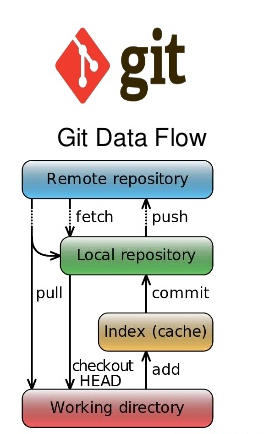
\includegraphics[scale=0.6]{git_workflow}
\caption{A summary of Git workflow taken from \href{http://www.slideshare.net/VinothKumarKannan/svn-vs-mercurial-vs-github}{here} }
\label{fig:git_workflow}
\end{figure}
Figure \ref{fig:git_workflow} encompasses a good chunk of what you need to know about Git. The following sections will show you two important examples:
\begin{itemize}
\item [1.] How to create a local repository on your computer, a remote repository on Github and synchronize the two. In particular, the \textit{init}, \textit{add}, \textit{commit} and \textit{push} commands will be exemplified. 
\item [2.] How to contribute to code in a collaborative environment.
\end{itemize}
\subsection{How to set up a local/remote repository}

\subsubsection{Create the local repository}
We begin by opening a terminal window into the folder where we want to create our repository. In this example, the repository will be in a folder named \textit{NewStudentHandout} located in the \textit{Documents} folder of a Unix system. On a Mac, the terminal command \textit{pwd} would return 
\textit{/Users/my\_username/Documents/NewStudentHandout} when executed from \textit{NewStudentHandout}. Once we have made sure that the window terminal is in the right folder, let's type
\begin{lstlisting}[language=bash, caption=Creation of the local repository]
git init
\end{lstlisting}
If everything goes well, the following should appear on the terminal window:
\begin{lstlisting}[language=bash, caption=Successful git init message ]
Initialized empty Git repository in /Users/bbercovici/Documents/NewStudentHandout/.git/
\end{lstlisting}
This command initiates the local git repository by creating the hidden directory \textit{./git} and populates it with a number of configuration files. These files are the backbone of your local repository, so make sure not to alter them.\\
As noted by Git, our local repository is empty. Note that the working directory content is unrelated to the local repository content as those are two separate entities as shown on Figure \ref{fig:git_workflow}. We thus have to use \textit{add} to add files to the index cache, and \textit{commit} this index to have those files added to our local repository.\\
Let us start with the \textit{add} command. It can be used in two different ways, as shown below (assuming that \textit{myfile.txt} does exist in the working directory):
\begin{lstlisting}[language=bash, caption=Add files to the cache ]
git add myfile.txt
# the index cache only contains myfile.txt
git add *
# the index cache now contains all files in the working directory that were not excluded in .gitignore 
\end{lstlisting}
Another useful command is \textit{status}, which highlights files depending on whether they have been modified since the last commit. Since \textit{git status} lists myfile.txt in green, we are now ready to commit it to the local repository using the following command:
\begin{lstlisting}[language=bash, caption=commit files to the local repository ]
git commit -m "first commit: myfile.txt added to the local repo"
\end{lstlisting}
The "-m" options allows us to append a message to the commit. After the content of the local repository is pushed to remote repository, the other developers will be able to read the message and quickly understand what this commit was about.

\subsubsection{Create an account on Github}
The title of this section is quite self-explanatory. Make sure you remember your username/password as you will need them shortly!
\subsubsection{Create the remote repository on Github}
Log on to Github and click on "New repository" in the drop-down list next to your profile picture as show on Figure \ref{fig:new_repo}.
\begin{figure}[H]
\centering
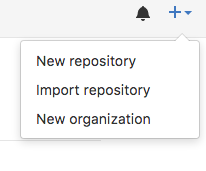
\includegraphics[scale=0.5]{new_repo}
\caption{New repository}
\label{fig:new_repo}
\end{figure}

The following window (shown on Figure \ref{fig:new_repo_settings}) allows you to choose several important settings for your remote repository.
\begin{figure}[H]
\centering
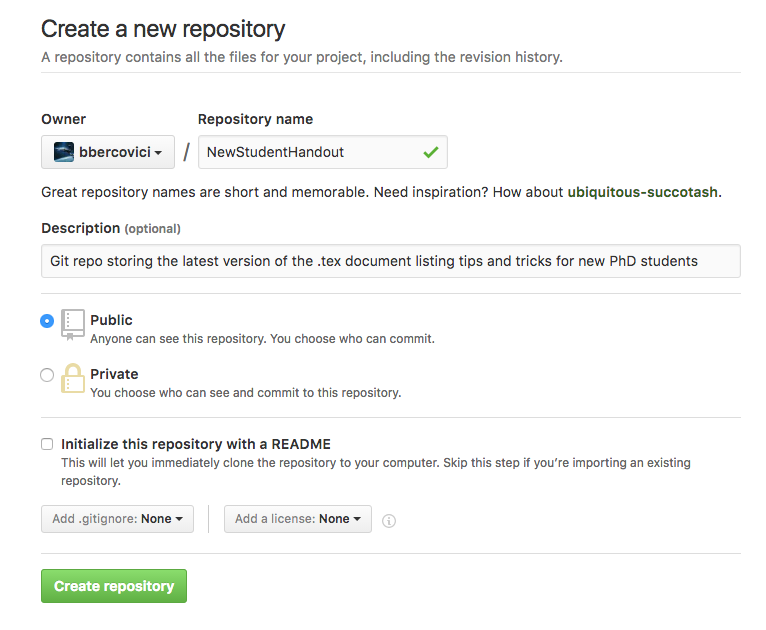
\includegraphics[scale=0.6]{new_repo_settings}
\caption{New repository settings}
\label{fig:new_repo_settings}
\end{figure}

\begin{itemize}
\item Choose whether the repository will be made public or private (the latter being only available if you have upgraded to a premium account).
\item Initialize the repository with a README.md file. \\\textcolor{red}{Leave this box unchecked if your local repository is already created, as this file can be added later on manually without risking conflicts}
\item Add a .gitignore file. This file lists all the file extensions that must be ignored by Git. Especially handy if there are specific file extensions that you never want to see included in a commit.
\item Add a license file.
\end{itemize}
When you are ready, simply click on Create Repository and proceed to the next step.
\subsubsection{Connect the local repository to the remote repository}
You should now be seeing the same page as on Figure \ref{fig:setup_options}. 

\begin{figure}[H]
\centering
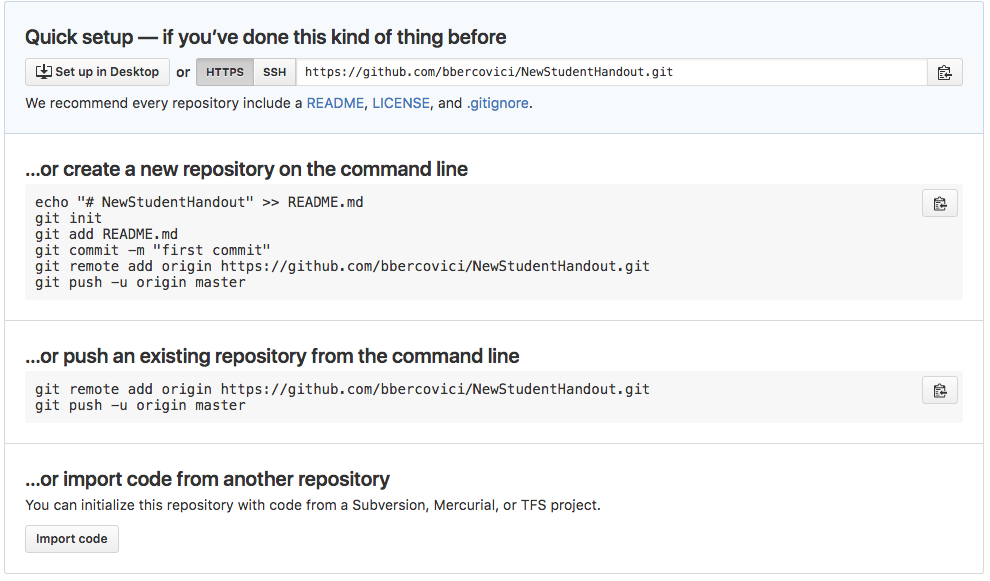
\includegraphics[scale=0.4]{setup_options}
\caption{Final setup options}
\label{fig:setup_options}
\end{figure}
The third option is what we want to do, since we have already created a (local) repository. We can copy and paste the two lines under "...push an existing repository from the command line" into our terminal. Start with the following:
\begin{lstlisting}[language=bash, caption=Add the remote repository location ]
git remote add origin https://github.com/bbercovici/NewStudentHandout.git
\end{lstlisting}
This will add the remote repository address to one of the hidden configuration files. Finally, push the local repository to the remote.

\begin{lstlisting}[language=bash, caption=Push the local repository to the remote ]
git push -u origin master
\end{lstlisting}

We are now all set! We can keep working in our local directory, add files containing new content to the index using \textit{git add}, commit the changes to the local repository using \textit{git commit}, and finally pushing the changes to the remote using \textit{git push origin master} (note that the -u option was not used here). Now is also the time to create a .gitignore file and a README.md file.
\subsection{Contribute to code in a collaborative environment}

Test